\section{Benutzerhandbuch}
\subsection{Einführung}
In diesem Dokument wird die Benutzerfunktionen von TouchDown‚Ñ¢ für
Android-Geräte beschrieben. Es dient als Benutzerhandbuch für die
unterschiedlichen Funktionen der Anwendung und soll Ihnen beim
Ausführen von häufigen Aktionen innerhalb der Anwendung Hilfe bieten.
Die Installation und Konfiguration von TouchDown wird in einem
separaten Dokument behandelt. Weitere Informationen finden Sie im
Installations- und Konfigurationshandbuch.
HINWEIS: In diesem Dokument wird vorausgesetzt, dass TouchDown
bereits installiert, konfiguriert und der vollständige Funktionsumfang
aktiviert wurde.
\begin{figure}[h]
	\centering
	\includegraphics[scale=0.5]{03_Bedienungsanleitung/img/appstore.jpg}
	\caption{eine Grafik ohne Sinn und Verstand}
	\label{img:grafik-dummy}
\end{figure}

\subsection{Hauptbildschirm}

\begin{wrapfigure}{r}{0.5\textwidth}
  \begin{center}
    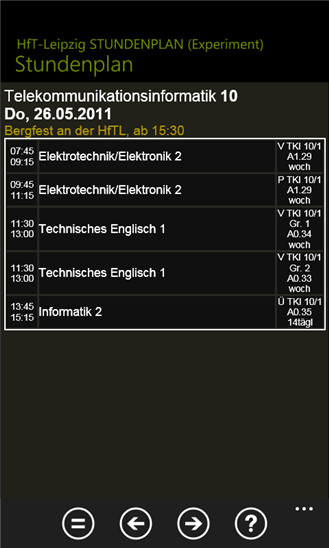
\includegraphics[width=0.3\textwidth]{03_Bedienungsanleitung/img/hftlapp.png}
  \end{center}
  \caption{HFTL-APP©gemeinfrei}
  \label{reaper}
\end{wrapfigure}

Sobald Sie das Programm installiert und Ihr Konto konfiguriert haben,
können Sie TouchDown starten, indem Sie auf dem Startbildschirm des
Geräts auf das TouchDown-Symbol tippen.
\\
Am Bildschirm „E-Mail“ (Abbildung 3) wird die Kopfzeile jeder E-Mail in
einer Listenansicht angezeigt. Ein grüner Balken auf der linken Seite der E
Mail zeigt an, dass es sich um eine ungelesene E-Mail handelt. Der Betreff
der E-Mail wird oben angezeigt, darunter folgt in grau der Name des
Absenders und anschließend der Nachrichtentext. Auf der rechten Seite
wird der Zeitstempel der E-Mail angezeigt. Ganz links befindet sich ein
leeres Kontrollkästchen. Wenn Sie auf das Kontrollkästchen tippen, wird
dieses grün hervorgehoben, und Sie können mehrere E-Mails gleichzeitig
verschieben oder löschen. Sobald die entsprechenden Elemente ausgewählt
sind, können Sie auf „Menü“ tippen und die gewünschte Aktion auswählen.

\subsection{E-Mail}

Am Bildschirm „E-Mail“ (Abbildung 3) wird die Kopfzeile jeder E-Mail in
einer Listenansicht angezeigt. Ein grüner Balken auf der linken Seite der E
Mail zeigt an, dass es sich um eine ungelesene E-Mail handelt. Der Betreff
der E-Mail wird oben angezeigt, darunter folgt in grau der Name des
Absenders und anschließend der Nachrichtentext. Auf der rechten Seite
wird der Zeitstempel der E-Mail angezeigt. Ganz links befindet sich ein
leeres Kontrollkästchen. Wenn Sie auf das Kontrollkästchen tippen, wird
dieses grün hervorgehoben, und Sie können mehrere E-Mails gleichzeitig
verschieben oder löschen. Sobald die entsprechenden Elemente ausgewählt
sind, können Sie auf „Menü“ tippen und die gewünschte Aktion auswählen.

\begin{figure}[h]
	\centering
	
\includegraphics[scale=1.0]{03_Bedienungsanleitung/img/perfekt.jpg}
	\caption{eine Grafik ohne Sinn und Verstand}
	\label{img:grafik-dummy}
\end{figure}
